This section introduce the principal ideas of \oursystem.
namely the
formation of a two-dimensional representation of a three-dimensional world, and what
we may deduce about the 3D structure of what appears in the images.

The drop from three-dimensional world to a two-dimensional image is a projection
process in which we lose one dimension. The usual way of modelling this process is
by central projection: in which a ray of light
from a point in the world passes through the lens of a camera and impinges on a film or
digital device, producing an image of the point. Ignoring such effects as focus and lens
thickness, a reasonable approximation is that all the rays pass through a single point,
the centre of the lens.

In a calibrated camera, it is possible to determine the angle between the two rays
back-projected from two points in the image.

Consequently, knowing the IAC, one can measure the angle between rays by direct
measurements in the image.

So far we have considered the reconstruction of a scene, or transfer, for images taken
with a set of uncalibrated cameras. For such cameras, important parameters such as
the focal length, the geometric centre of the image (the principal point) and possibly
the aspect ratio of the pixels in the image are unknown.

So far, we have discussed projective reconstruction, which is all that is possible without
knowing something about the calibration of the cameras or the scene.

it is only the motion of the camera that is important here; we do not need to
reconstruct the scene,

3D to 2D camera projection. Given a set of points Xi in 3D space, and a set
of corresponding points xi in an image, find the 3D to 2D projective mapping
that maps Xi to xi. Such a 3D to 2D projection is the mapping carried out by a
projective camera, as discussed in chapter 6.

Shape is distorted under perspective imaging.????



Two types of vision-based localization are implemented by SocialLens for diverse mobile devices:
 the monocular-vision localization and binocular-vision localization.


\begin{figure}[t!]
\centering
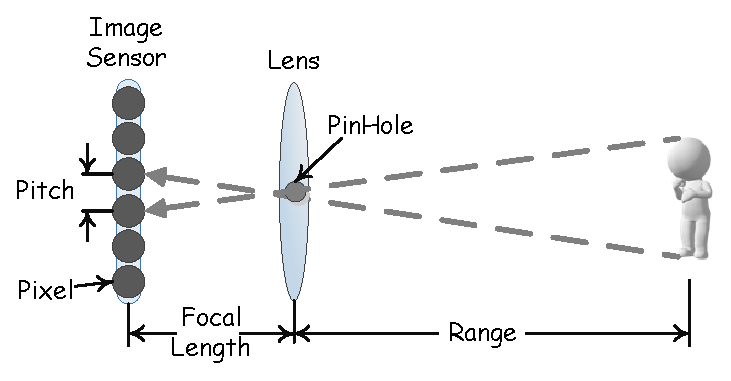
\includegraphics[width=0.9\linewidth]{pinhole.eps}
\caption{Pinhole geometric model of monocular camera.}\label{fig_pinhole}
\end{figure}


\paragraph{Monocular vision based localization}
So far, many smart phones has one camera lens and the photos are in 2D format.
Many exiting work, \eg \cite{Anat08,Adelson92},
 estimate the position(depth or distance) of people by analyzing the 2D image.
Most of them requires special camera, \eg professional-quality camera,
 plenoptic camera or camera with coded aperture.
Others requires the measured object to be far away from the camera, \eg a building.
SocialLens uses the low-quality perspective camera of the commercial mobile device
 to estimate the depth of the people in a image.

The first monocular cue of depth is \emph{elevation}.
Basically��in a image people who are closer to the upper horizon are farther away,
  and people who are closer to the lower horizon are closer to the camera.
SocialLens decides the relative depth of people by elevation using the face detection, upbody detection and whole body detection results.
Figure~\ref{fig_position} shows the possible position situations.
In the cases with check marks, the relative depth can be decided,
 but in cases with question marks, the relative depth is uncertain,
 \eg, a person closer but much higher than another farther person.

So we need the relative depth of people in the uncertain cases,
 as well as more accurate ranging result.
SocialLens uses the geometric model of classical pinhole camera, as shown in Figure  ~\ref{fig_pinhole},
  which is the model for most camera systems.
Let $p$ be the \emph{pixel pitch} between adjacent pixels on the image sensor of camera.
Then we have $p=\frac{sensor height (mm)}{image height(pixel)}$, which is a intrinsic parameters of a camera.For example, on the image sensor of EVO 3D, $P=1.75 \mu m$.
The focus length $f$ is also a intrinsic parameter, which is the distance from the ''pinhole''
 to the image sensor .
Let $h$ denote the real size of an object outside of the camera,
 and $a$ is its apparent size in the image in pixels.
$r$ is the range or distance from the object to the camera.
Then these variables follow the relationship:
\begin{equation}
\frac{a\cdot p}{f}=\frac{h}{r}.
\end{equation}
Using this model, if some absolute size of people is known,
 an absolute distance can be calculated.
Based on our detection method, the absolute size of people could be eye distance,
 shoulder width and height.
If two object are known to be the similar size but their absolute size is unknown (\eg. the eye distance), relative size in the vision can provide information about the relative depth of the two objects.
This pinhole model based method can provide sub-meter level accurate,
 when people are within 10 meters range of the camera.
The inaccuracy are mainly caused by the distortion of lens
 and the deviation of the human feature detection.


Motion also provide cues for depth, \eg the motion parallax \cite{Ferris95}(when the observer moves, nearby things pass quickly, while far off objects appear stationary).
If information about the direction and velocity of movement is known,
 motion parallax can provide absolute depth information.
The motion status is acquired from the sensors of the observer's phone.
By tracking the people, we can update the ranging of them.






%Of these various cues, only the depth from motion provide absolute distance information.
%All other cues are relative (i.e., they can only be used to tell which objects are closer relative to others). Stereopsis is merely relative because a greater %or lesser disparity for nearby objects could either mean that those objects differ more or less substantially in relative depth or that the foveated object is %nearer or further away (the further away a scene is, the smaller is the retinal disparity indicating the same depth difference).

\begin{figure}[t!]
\centering
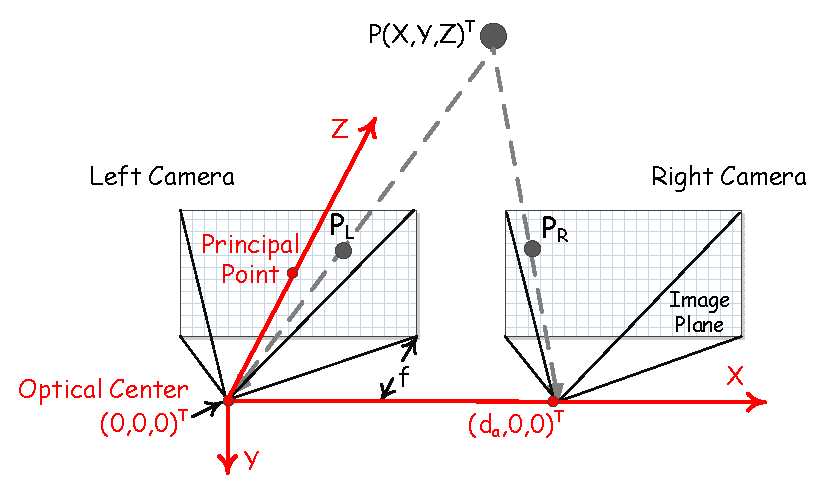
\includegraphics[width=0.95\linewidth]{twoview.eps}
\caption{Model of two aligned cameras capturing rectified images for depth estimation.}\label{fig_twoview}
\end{figure}

\paragraph{Binocular vision based localization}
Recently more commercial smart phones support 3D views,
 like HTC Evo 3D and LG Optimus 3D.
A stereo camera with two aligned lenses simulates human binocular vision
 and gives the ability to capture 3D images for making stereoviews and range imaging.
The binocular vision based localization
 requires input from two lenses to estimate ranging of objects.
The most important binocular cue is stereopsis or retinal (binocular) disparity.
It yields depth from binocular vision through exploitation of parallax.
By using two images(left and right) of the same scene obtained from slightly different angles,
 SocialLens triangulates the distance to an people with a high degree of accuracy.
Intuitively, if an object is far away, the disparity of that image falling on both retinas will be small; if the object is close or near, the disparity will be large.
SocialLens uses the following steps to estimate a person's distance to the camera:
    \begin{enumerate}[1)]
    \item Calibration: calibrate a camera with the given chessboard image.
    Because there may be a significant distortion.
    Luckily, these are constants and with a calibration and some remapping we can correct this. \item Human detection: detect the faces/upper body/whole body in both left and right images.
    \item Correspondence problem: figure out which points set of the left image correspond to which points set of the right image, here the image points sets are the pixel sets of faces/upperbody/whole body.
    \item Stereo triangulation: range people based on stereo triangulation.
    \end{enumerate}
Figure~\ref{fig_twoview} shows the geometry model of a stereo camera with two
 aligned lenses.
Optical center is the center of the perspective projection.
The line perpendicular to the image plane passing through the optical center
 is the optical axis.
The intersection point of the optical axis and the image plane is called the principal point.
Without loss of generality, the world coordinate system is selected such that
 its origin is located at the optical center of the left camera
 and the Z-axis is collinear to the optical axis, as shown in Figure~\ref{fig_position}.
$P$ is a 3D Euclidean point $(X,Y,Z)^T$ captured by two cameras
 and the two corresponding projected pixels are $P_L$ and $P_R$,
 whose pixel positions are $(x_L,y_L)$ and $(x_R,y_R)$ respectively.
Let the principal point of left camera be $(o_x,o_y)^T$.
Then the projection of $P$ onto the image plane of the left camera is
\begin{equation}
x_L = \frac{Xf}{Z}+o_x, y_L = \frac{Yf}{Z}+o_y.
\end{equation}
Expressed in matrix:
\begin{equation}
\lambda_L \begin{pmatrix}x_L \\ y_L \\ 1 \end{pmatrix} = \begin{pmatrix}f & 0 & o_x\\0 & f & o_y\\ 0 & 0 & 1 \end{pmatrix} \begin{pmatrix}X \\ Y \\ Z\end{pmatrix}.
\end{equation}
$\lambda_L$ is a scaling factor.
Let $K=\begin{pmatrix}f & 0 & o_x\\0 & f & o_y\\ 0 & 0 & 1\end{pmatrix}$,
when the origin of the pixel coordinate system corresponds to the principal point,
 $(o_x,o_y)^T=(0,0)^T$.
The right camera is located on the $X$ axis
 and its optical center is $(d_a,0,0)$.
Because both cameras are identical,
 so we have:
\begin{equation}
\lambda_R \begin{pmatrix}x_R \\ y_R \\ 1 \end{pmatrix} = K \begin{pmatrix}X \\ Y \\ Z\end{pmatrix} - K  \begin{pmatrix}d_a \\ 0 \\ 0\end{pmatrix}.
\end{equation}
Then the relationship between two corresponding pixels $P_L$, $P_R$ and the depth Z of $P$ is
\begin{equation}
\begin{pmatrix}x_R \\ y_R \end{pmatrix} = \begin{pmatrix} {x_L-\frac{f \cdot d_a}{Z}} \\ y_L \end{pmatrix}.
\end{equation}
So the depth of point $P$ is
\begin{equation}
  Z=\frac{f \cdot d_a}{Disparity}.
\end{equation}
